\documentclass{beamer}

\usepackage{ctex}
\usepackage{graphicx} % Allows including images
\usepackage{booktabs} % Allows the use of \toprule, \midrule and \bottomrule in tables
\usepackage{biblatex}
\usepackage{xcolor}
\usepackage{algorithm,algorithmic} 
\usetheme{Warsaw}
\usefonttheme[onlymath]{serif}

%Information to be included in the title page:


% \AtBeginSection[]
% {
%     \begin{frame}
%         \frametitle{Table of Contents}
%         \tableofcontents[currentsection]
%     \end{frame}
% }
\AtBeginSubsection[]{
	\begin{frame}
		\frametitle{目录}
		\tableofcontents[currentsubsection]
	\end{frame}
}
\title{并行单纯形法}
\author{张博阳 211840196}
\date{June 2024}

\begin{document}

\frame{\titlepage}

\begin{frame}
    \frametitle{目录}
    \tableofcontents
\end{frame}

\section{单纯形法}
\subsection{线性规划标准型}
\begin{frame}
    \frametitle{线性规划标准型}
    单纯形法适用于求解下述线性规划标准型:
    \begin{align*}
         & \min\ f=c^\mathrm{T}x \\
         & \ \mathrm{s.t.}\ Ax=b \\
         & \qquad x \ge 0
    \end{align*}
    其中$A\in M_{m\times n}(\mathbb{R}),b \ge 0 \in \mathbb{R}^m,c \in \mathbb{R}^n,x \in \mathbb{R}^n$.
\end{frame}

\begin{frame}
    \frametitle{线性规划标准型}
    问题的解有三种情形:
    \begin{itemize}
        \item 存在有界解
        \item 存在无界解
        \item 无解
    \end{itemize}
\end{frame}

\begin{frame}
    \frametitle{线性规划标准型}
    问题的解有三种情形:
    \begin{itemize}
        \item \textbf{存在有界解}
        \item 存在无界解
        \item 无解
    \end{itemize}
\end{frame}

\subsection{单纯形法执行步骤}
\begin{frame}
    \frametitle{单纯形法执行步骤}
    \begin{itemize}
        \item 数据初始化,开辟存储判别数的$n$维数组,\underline{指定初始基变量}
        \item 对于每一基变量($O(m)$)
              \begin{itemize}
                  \item 对基变量执行单位化($O(n)$)
                  \item 对单纯形表执行列消去运算($O(mn)$)
              \end{itemize}
        \item 计算各变量判别数$\gamma_j=c_j-\sum_{i\in base}c_it_{ij}\quad$($O(mn)$)
        \item 检查各判别数($O(n)$)
              \begin{itemize}
                  \item 若判别数均不为负,表明最优解已求得,退出迭代
              \end{itemize}
        \item 若存在负判别数,选择负判别数中绝对值最大者为进基变量,选择该变量所在列中$\dfrac{t_{i,n+1}}{t_{ij^*}}$为正的最小行对应的基变量为出基变量($O(m)$),更新基变量,转步骤2
              \begin{itemize}
                  \item 若各行均不为正,表明存在无界解,退出迭代
              \end{itemize}
    \end{itemize}
\end{frame}

\section{并行化及其代码实现}
\subsection{并行单纯形表迭代}
\begin{frame}
    \frametitle{并行单纯形表迭代}
    \begin{itemize}
        \item 由于单纯形法是高度顺序化的,因此难以完全并行实现
              \begin{itemize}
                  \item 判别数的计算依赖于换基运算后得到的单纯形表
                  \item 进出基的选择依赖于判别数的计算
                  \item Barriers调用时机
              \end{itemize}
        \item 考虑在每次迭代内部使用并行技术加速计算
              \begin{itemize}
                  \item 仅在列消去($O(m^2n)$)和判别数($O(mn)$)计算使用并行技术
                        \begin{itemize}
                            \item 基变量确定的情况下,各行的消去是彼此独立的
                            \item 判别数计算是各变量间独立的
                        \end{itemize}
                  \item 其他步骤仍顺序执行
              \end{itemize}
    \end{itemize}
\end{frame}

\subsection{类的设计及代码框架}
\begin{frame}
    \frametitle{类的设计及代码框架}
    \begin{figure}[H]
        \centering
        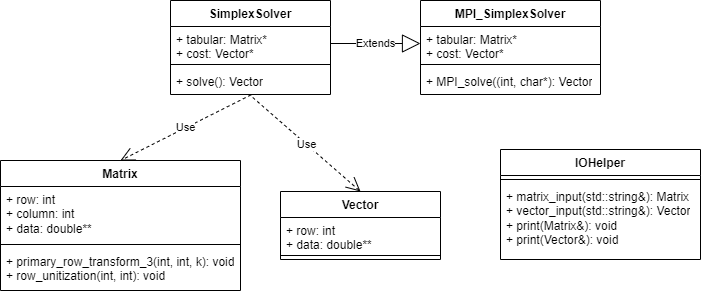
\includegraphics[width=1\linewidth]{MPI_SimplexSolver.drawio.png}
        \caption{\texttt{MPI\_SimplexSolver}类图}
    \end{figure}
\end{frame}

\begin{frame}
    \frametitle{类的设计及代码框架}
    \begin{figure}[H]
        \centering
        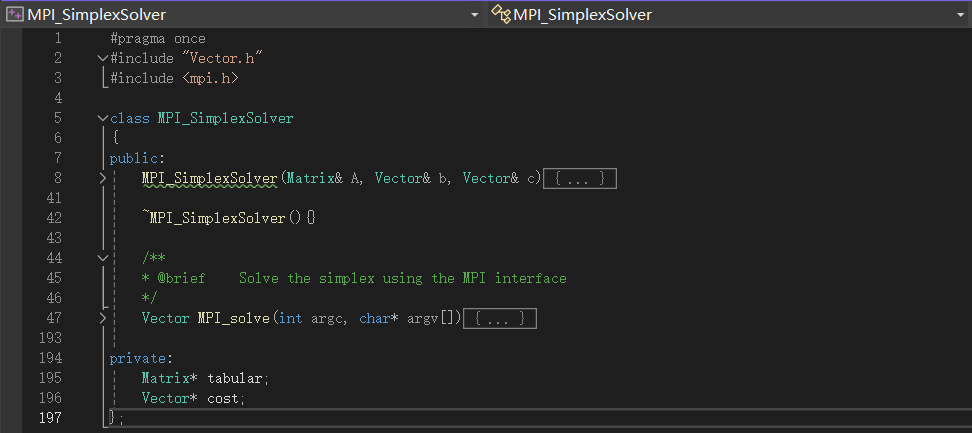
\includegraphics[width=1\linewidth]{MPI_SimplexSolver.png}
        \caption{核心类\texttt{MPI\_SimplexSolver}结构}
    \end{figure}
\end{frame}

\begin{frame}
    \frametitle{类的设计及代码框架}
    \begin{figure}[H]
        \centering
        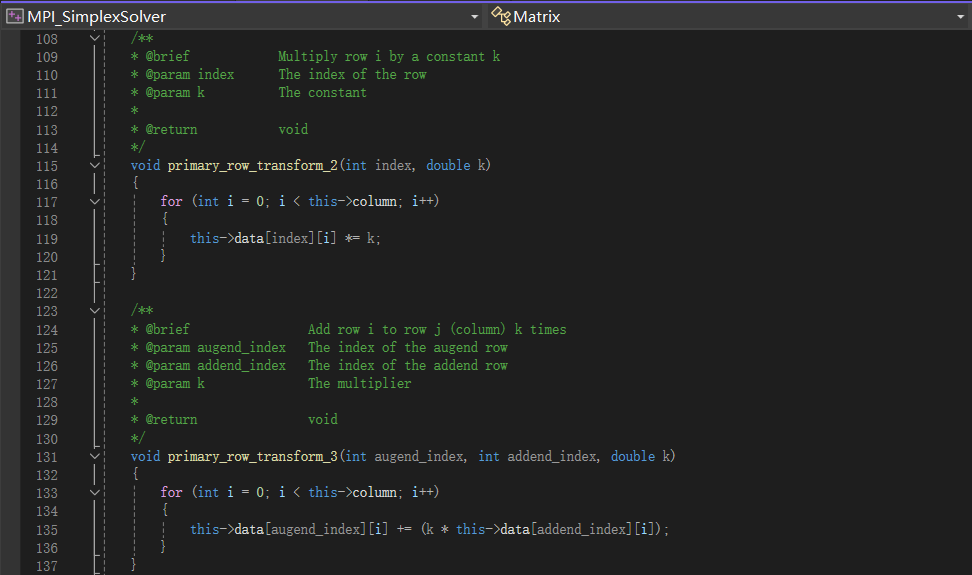
\includegraphics[width=1\linewidth]{Matrix1.png}
        \caption{类\texttt{Matrix}结构}
    \end{figure}
\end{frame}

\begin{frame}
    \frametitle{类的设计及代码框架}
    \begin{figure}[H]
        \centering
        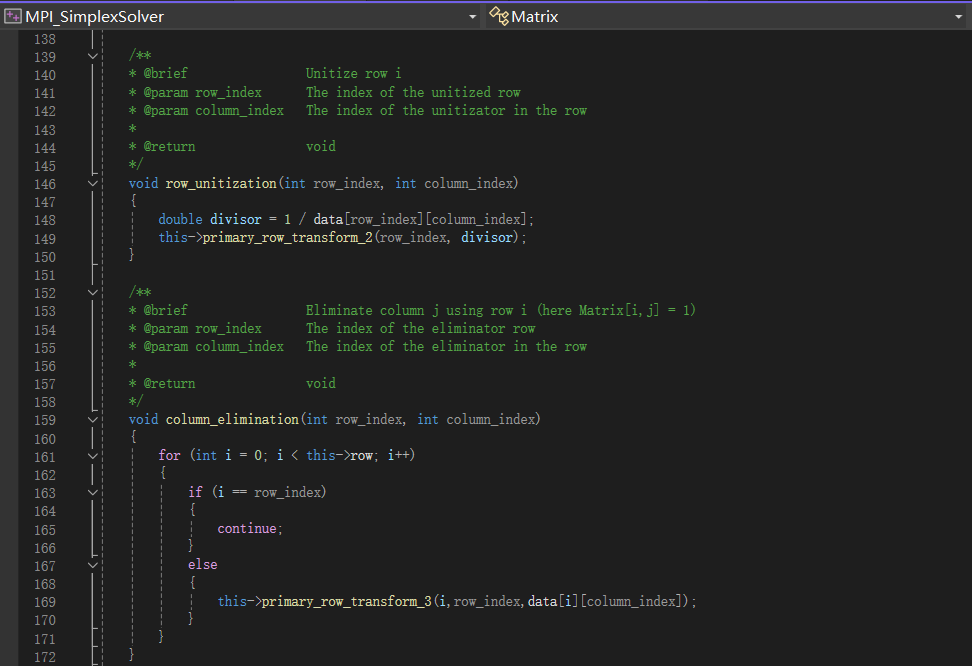
\includegraphics[width=1\linewidth]{Matrix2.png}
        \caption{类\texttt{Matrix}结构}
    \end{figure}
\end{frame}

\end{document}
